\documentclass[../documentation.tex]{subfiles}
 
\begin{document}
\section{Sakkalgoritmus beágyazása}
A robotprogramhoz felhasznált sakkalgoritmusok és főbb Java osztályok alapja egy versenyre készített, nyílt forráskódú sakk alkalmazás \cite{chessgui}. 2005-ben Arwid (Arvydas) Bancewicz első helyezést ért el ezzel az alkalmazásával az OBEA Számítógépes Programozó Versenyen (\angol{OBEA Computer Programming Contest}) 17 évesen. Az általa készített program rendelkezik grafikus felhasználói felülettel (továbbiakban GUI - \angol{Graphical User Interface}), a forráskód nagy része ennek megfelelő működtetéséhez lett megírva.

A szakdolgozat keretében megvalósított projektem során külön a sakk alkalmazáshoz felhasználói felületet létrehozni nem volt szükségszerű. A robotprogram továbbfejleszthető olyan formában, hogy folyamatosan kijelezze a jelenlegi sakkállást, így még inkább nyomon követhető a játék menete, így megkönnyítve a továbbfejlesztést. Ezen a felületen keresztül akár tetszőleges felállást lehetne konfigurálni a játék kezdetéhez.

A sakkprogram beágyazásának első fő kihívása a GUI elhagyásával egy konzolalkalmazás létrehozása. A program forráskódja viszonylag hosszú, sok osztály lett implementálva különböző csomagokba rendezve (12 csomag és ezeken belül 93 osztály). A program működésének megértéséhez jó kiindulási pont a mellékelt README fájl és a ``\angol{program documentation}'' mappában található szotver leírás (\angol{Software Documentation.doc})\cite{chessgui}. Habár ezek főként a GUI működését taglalják, az ehhez tartozó főprogram kódjából a meghívott függvények alapján ki lehet következtetni a működés struktúráját. Ezen felül a Java osztályoknak és az egyes csomagoknak beszédes nevük van, például a következő sakklépést az \angol{algorithm} (algoritmus) csomagban található különböző algoritmusokra alapozott osztályok metódusai határozzák meg.

A szakdolgozathoz felhasznált csomagok az alábbiak (ezeken belül is bizonyos funkciók ki lettek kapcsolva, de ezek jelentik a program magját):
\begin{itemize}
	\item chess.algorithm: Ebben a csomagban kerültek implementálásra a különböző sakkalgoritmusokat meghívó és végrehajtó utasítások. Ezen felül itt lettek implementálva az bábuk lehetséges lépései.
	\item chess.core: Ez a csomag tartalmazza a sakkhoz szorosan kötődő osztályokat, metódusokat (pl.: bábuk elhelyezkedése a táblán).
	\item chess.properties: Itt találhatóak a programozott sakkjáték szempontjából praktikus funkciók (pl.: játék jelenlegi állása, játékosok neve stb.).
\end{itemize}

\subsection{A chess.algorithm csomag - az algoritmusok működtetője}
A programban az alábbi sakkalgoritmusok lettek implementálva:
\begin{itemize}
	\item Alfa-béta vágás (AlphaBeta.java)
	\item Minimax elv (MiniMax.java)
	\item NegaScout algoritmus (NegaScout.java)
	\item Principal variation search (PrincipalVariation.java)
	\item Kvázi véletlenszerűen választott szabályos lépés (RandomGen.java)
\end{itemize}

A sakkprogram alapbeállításként az Alfa-béta vágást használja. Az Alfa-béta vágás egy olyan kereső algoritmus, amely igyekszik csökkenteni a minimax algoritmus keresési fájában lévő kiértékelt elemek számát. Ezt a módszert gyakran alkalmazzák kétszemélyes játékok (pl.: amőba, sakk, go, stb.) esetén gépi játékos programozására. Egy adott lépés kiértékelését akkor szakítja meg teljesen, ha legalább egy válaszlépés bebizonyítja, hogy a lépés rosszabb, mint a korábban vizsgált lépés. Az ilyen lépések további vizsgálata felesleges. Ha egy hagyományos minimax fára alkalmazzák, akkor ugyanazt a lépést adja majd vissza, mint amit a minimax algoritmus adna, de kimetszi azokat az ágakat a fában, amik a kimenetet nem befolyásolják.\footnote{Szöveg forrása angol nyelven: https://en.wikipedia.org/wiki/Alpha\%E2\%80\%93beta\_pruning}

\begin{figure}[h]
\centering
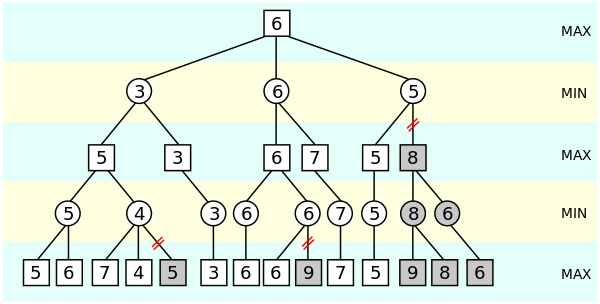
\includegraphics[scale=0.55]{alphabeta}
\caption{Az alfa-béta vágás szemléltetése. A kiszürkített részfák vizsgálata felesleges (a lépések jobbról balra történő kiértékelésekor). A max és min szintek reprezentálják a játékos, illetve az ellenfelének a lépéseit. \protect\footnotemark}
\label{fig:alphabeta}
\end{figure}
\footnotetext{A kép forrása: https://upload.wikimedia.org/wikipedia/commons/thumb/9/91/\\AB\_pruning.svg/600px-AB\_pruning.svg.png}

Az algoritmus két változót értékel ki minden lépésben, alfát és bétát. Az alfa érték reprezentálja azt a minimum pontszámot, amely az u.n. `maximalizáló' játékos számára már biztosítva van, illetve a béta érték az a maximum pontszám, ami az u.n. `minimalizáló' játékos számára biztosított. Kezdetben alfa értéke negatív végtelen, béta pozitív végtelen, azaz mindkét játékos a saját legrosszabb lépésével indít. A fa rekurzív vizsgálata során folyamatosan változik az értékük a játékosok által garantáltan elérhető értékekre. Amint a béta érték az alfa alá csökken az azt jelenti, hogy ez az állás (ha mindkét játékos részéről a legjobb lépéseket tételezzük fel) nem állhat elő, így további vizsgálatuk felesleges.

Az algoritmusokat a sakk szabályaihoz és sajátosságaihoz a MoveAlgorithm illeszti. Ez az osztály az alábbi funkciókat tartalmazza (egyéb kiegészítő, teszteléshez megírt függvényeken felül):
\begin{itemize}
	\item Definiálja az egyes bábuk lehetséges lépéseit mezőkre lebontva, tehát az erre vonatkozó metódusok pontosan megadják, hogy az egyes bábuk melyik mezőkről melyikekre léphetnek. Példának okáért a gyalog esetén külön a fehér bábukra és külön a feketékre is meg van határozva (getPawnMoves(Coord c) függvény), hogy a kiindulási pontjukról az ellenfél irányába egyet vagy kettőt is léphetnek. Bármely más esetben 1-et léphetnek előre (az ütéseket külön függvények definiálják, ezek elkülönítése a robotprogramozás esetén is kifejezetten előnyös).
	\item Az egyes bábuk lehetséges ütéseit külön függvények határozzák meg. A gyalog kivételével a többi bábunál ez megegyezik az előző pontban leírt lépésekkel.
	\item A bábuk játékhelyzettől függő összes lehetséges lépését, ütését a `getRealMoves', a `getRealAttacks' és a `getRealAll' függvények adják vissza. Ezek kizárján azon lépéseket, melynél az adott játékos királya a lépés előtt és utána is sakkban áll. Ezt úgy vizsgálja meg a program, hogy adott játékállásban ``meglépi'' a kívánt lépést, majd ellenőrzi, hogy a király sakkban maradt-e.
	\item Itt találhatóak még az egyes játékállások ``költségét'' meghatározó függvények, amelyek által visszaadott értékek az algoritmusok működtetésének alapjait jelentik.
\end{itemize}

\subsection{A chess.core csomag - a játék magja}
A chess.core csomag definiálja az algoritmusok működtetéséhez nem szorosan kapcsolódó osztályokat. A fő fájl a ChessGame.java, ennek segítségével lehet egy játékot elkezdeni. A példányosításakor az alábbi inicializáló lépések futnak le:

\begin{enumerate}
	\item A játék állapota inicializáltra változik (a játékállapotokról a chess.properties csomag kapcsán lesz bővebben szó).
	\item Alapértelmezetten az Alfa-béta kereső algoritmus kerül beállításra. Ezt a játék során bármikor lehet módosítani a `setAlgorithm' függvény segítségével.
	\item A játékosok neve alapértelmezetten ``Black'' és ``White'', ezt is bármikor lehet módosítani a játék közben. Kiindulásként a fehér játékos az ember, a fekete a robotkar, de a program viszonylag könnyedén átalakítható ha ezt meg szeretnénk cserélni.
	\item A hagyományos sakkjátszmák során a játékosok egy sakkórát (\ref{fig:chessclock} ábra) használnak arra, hogy maximalizálják a játék idejét. Mindkét játékosnak előre meghatározott és beállított ideje van a gondolkozásra. Ha az adott játékos lépett, lenyom az órán egy kapcsolót, melynek hatására a másik játékos ideje telik addig, amíg ő is vissza nem kapcsolja az órát. A program két virtuális órát használ erre a célra, melyek indítása és megállítása automatikusan történik minden lépésnél.
\begin{figure}[h]
\centering
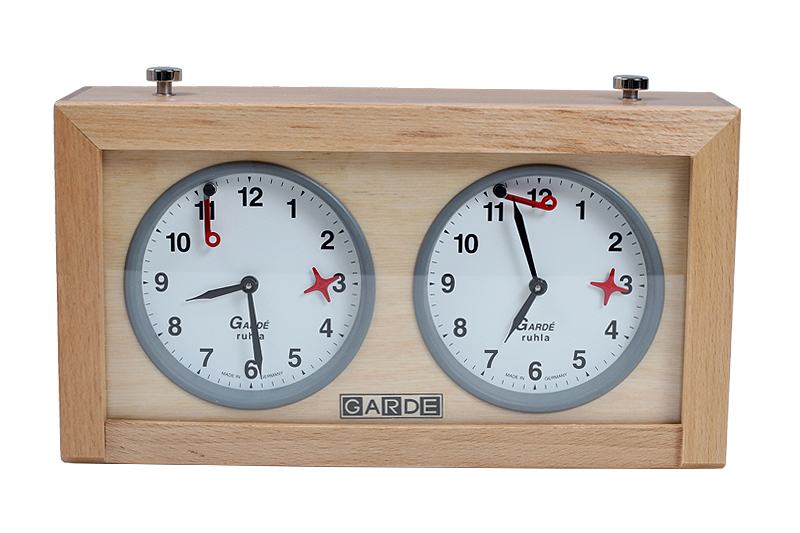
\includegraphics[scale=0.40]{chessclock}
\caption{Hagyományos játékokhoz használt sakkóra - a piros zászló leesése jelzi, ha a játékos ideje elfogyott \protect\footnotemark}
\label{fig:chessclock}
\end{figure}
\footnotetext{A kép forrása: https://www.polishchess.com/garde-analog-chess-clock-classic-p-161.html}
	\item A tábla és az alap felállás inicializálása a Board osztály példányosításával történik. Ez az osztály tartja számon, hogy melyik mezőn milyen bábu található, emellett praktikus okokból a két király jelenlegi helyzetét külön változókban tárolja.
\end{enumerate}

A bábuk pozíciója kapcsán külön érdemes kiemelni, hogy a pozíciót a bábuk koordinátája határozza meg. A lehetséges koordinátákat egy 8x8-as tömb jelképezi. A tömb [0,0] indexű eleme a tábla A1 mezője, a [7,7] pedig a H8 (\ref{fig:chessboard} ábra).

\begin{figure}[h]
\centering
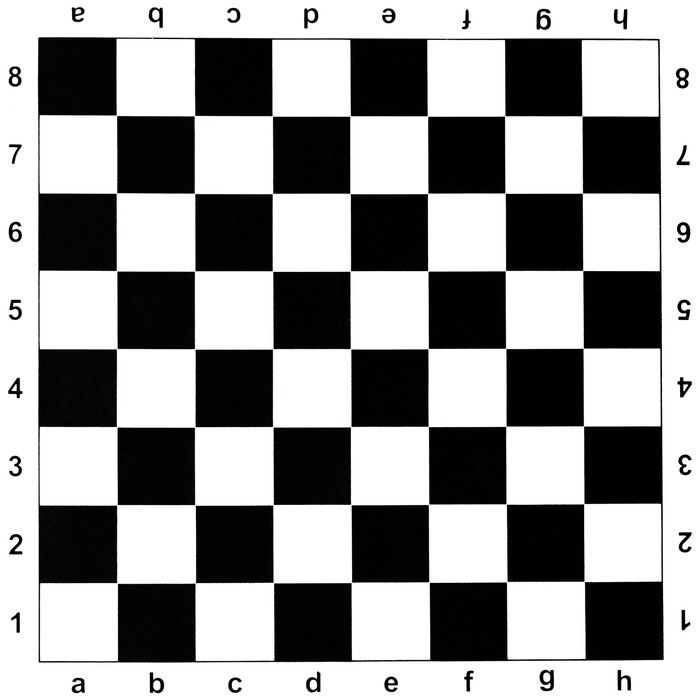
\includegraphics[scale=0.45]{chessboard}
\caption{A sakktábla mezőihez koordináták rendelése}
\label{fig:chessboard}
\end{figure}

Létrehozni lépést a Move osztály példányosításával lehet. A konstruktor egy kezdő és egy végponti $x$ és $y$ koordinátát vár, amelyek a bábu kiindulási- és végkoordinátái. Azt, hogy egy lépés szabályos volt-e úgy lehet ellenőrizni, hogy meghívjuk a sakkjáték példányunk `checkIfLegalMove' függvényét paraméterként átadva a lépést. Fontos, hogy a jelenlegi sakkjáték példányunkra hívjuk meg ezt a metódust, így biztos a pillanatnyi állás alapján dönt.

A lépések végrehajtása a szintén a ChessGame példányon belül implementált `movePiece' függvénnyel lehet. Ez első körben értelemszerűen megváltoztatja a bábuk helyzetét. Második lépésként az adott lépést hozzáadja a lépésekről vezetett listához (a ChessTableModel osztály segítségével). Ezek után a program átállítja, hogy ki a soron következő játékos, elindítja az óráját és ellenőrzi, hogy véget ért-e a játék, azaz mattot adott-e valamelyik fél.


\subsection{A chess.properties csomag - kiegészítő funkciók}
Ezen a csomagon tartalmaz számos a hagyományos sakkjáték végigjátszásához elengedhetetlen és néhány extra funkciót (a nélkülözhetetlen elemek ki lettek emelve a felsorolásban):

\begin{itemize}
	\item BoardParameters: továbbfejlesztés részeként a smartPAD-en meg lehetne jeleníteni a jelenlegi állást. Ehhez hasznos függvényeket és beállításokat tartalmaz ez az osztály.
	\item ChessColors: az előző pontban említett megjelenítéshez különböző színdefiníciókat bocsát rendelkezésre.
	\item ChessPreferences: segítségével el lehet menteni a jelenlegi játékhelyzetet. A program képes tetszőleges helyzetből kezdeni egy játékot, tehát ennek segítségével lehetséges egy játék későbbi folytatása.
	\item \textbf{GameParameters:} itt lehet beállítani az adott játékhoz használt sakkalgoritmus paramétereit (az algoritmus kiválasztása, kereső fa szintjeinek száma). Ezen felül itt lehet a játéknak címet adni, ez tárolja a játékosok nevét és azt, hogy melyik játékos helyett játszik a gép.
	\item \textbf{State:} meghatározza a játék jelenlegi állását (Vége van-e? Meg lett-e állítva? Inicializálva lett-e már? stb.).
\end{itemize}

\subsection{A sakkprogram kiegészítése a projekthez}
Ahogy \aref{fig:flowchart-chess} ábrán is látszik, a projekt megvalósításához a sakkprogramot össze kellett kötni a képfeldolgozást végző résszel és a robotvezérlővel. A képfeldolgozó rész meghatározza, hogy melyik mezőkön helyezkednek el a fehér bábuk, ez a sakkprogram bemenete. A kimenete pedig a szükséges lépés kezdő- és végpontja (pl.: [0,0] mezőről a [0,7] mezőre). Ezek fizikai koordinátákra transzformálása már a robotvezérlőn futó főprogramban történik. 

\begin{figure}[h]
\centering
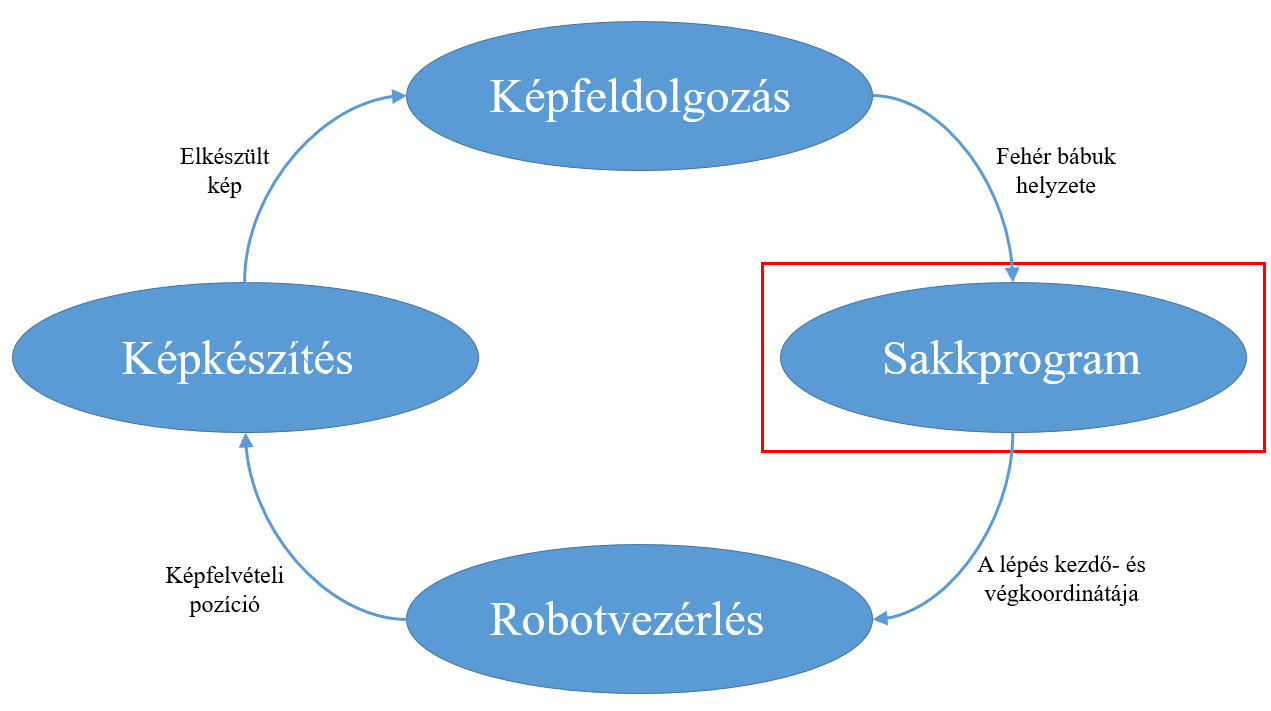
\includegraphics[scale=0.45]{flowchart-chess}
\caption{A sakkprogram helye a folyamatban}
\label{fig:flowchart-chess}
\end{figure}

A képfeldolgozás kimenete egy 8x8-as tömb (mátrix), amely indexelése megegyezik a sakkprogramnál bemutatott mezőindexeléssel (\ref{fig:chessboard} ábra). Ez a tömb az ember lépése utáni állapotban mutatja a bábuk elhelyezkedését. Ahhoz, hogy a megtett lépést meg lehessen határozni, ezt az állapotot össze kell vetni a lépés előttivel. A programben vezetett állást bármikor le lehet kérdezni (sakkjáték példány -> board -> b). A kapott elem egy 8x8-as tömb, amely egyes elemei vagy null értékűek vagy az ott található bábut írják le. Minden bábu esetén le lehet kérdezni, hogy fekete-e vagy fehér (white: bábu \angol{boolean} tulajdonsága - igaz ha fehér, hamis ha fekete). Ezek alapján létre lehet hozni egy olyan logikai értékeket tartalmazó tömbböt, amely formailag megegyezik a képfeldogozó rész által szolgáltatott tömbbel.

A lépés előtti és utáni tömböket a `FindMove' függvény értékeli ki. Elemenként hasonlítja össze a tömböket a program. Ha két elem megegyezik, az azt jelenti, hogy az ott lévő bábu nem mozdult el. Ha különbözik a két érték, akkor két eshetőség állhat fenn:

\begin{itemize}
	\item a bábu ellépett onnan (lépés után `false' a mező értéke) - ekkor ez a mezőkoordináta lesz a lépés kiindulópontja, vagy
	\item a bábu oda lépett (lépés után `true' a mező értéke) - ez a mező a lépés végpontja.
\end{itemize}

Két fehér bábu egy kör alatt csak sánszoláskor mozdulhat el. Ezt az eshetőséget a lépés meghatározásakor külön meg kell vizsgálni. Mivel a fekete bábuk pozícióját a sakkprogram követi, így nem igényel külön eljárás kialakítását az, ha a fehér játékos leüti a fekete egy bábuját. Ilyen esetben a leütőtt bábu pozíciójához a lépés előtt `false' érték tartozott, ezt a sakkprogram adja meg. A képfeldolgozó rész csak a fehér bábukat keresi (azokon van csak zöld jelölő), így az ütés után a mező értéke `true' lesz.

A lépés validálására érdemes meghívni a sakkjáték `checkIfLegalMove' függvényét mielőtt a lépést a programban végrehajtatnánk, mivel szabálytalan lépést is be lehetne vinni.







\end{document}